%
% sample.tex
% $Id: sample-10pt.tex,v 1.3 2006/08/10 01:53:43 johnh Exp $
%


% The default of sigplan-proc-varsize is 9pt, indented paragraphs (acm style)
% For Sensys or other 10pt conference, use the 10pt option
%\documentclass{sigplan-proc-varsize}
% options:
%\documentclass[9pt]{sigplan-proc-varsize}
\documentclass[10pt]{sigplan-proc-varsize}
%\documentclass[noindentedparagraphs]{sigplan-proc-varsize}



% % hack to avoid the ugly ACM paragraph definition
% % => can't leave blank line after this
% (remove comment for this hack)
 \renewcommand{\paragraph}[1]{\vskip 6pt\noindent\textbf{#1 }}


\usepackage{epsfig}
\usepackage{graphicx}
\usepackage[hyphens]{url}
\usepackage{hyperref}
\usepackage{algorithmic,comment}
\usepackage{epstopdf}
\usepackage{color}
\usepackage{authblk}

\nocopyrightspacetrue

\newcommand{\tabref}[1]{Table~\ref{#1}}
\newcommand{\figref}[1]{Fig.~\ref{#1}}
\newcommand{\eqnref}[1]{Equation~(\ref{#1})}
\newcommand{\secref}[1]{Section~\ref{#1}}
\newcommand{\redcolor}[1]{\textcolor{red}{#1}}
\newcommand{\bluecolor}[1]{\textcolor{blue}{#1}}

\newcommand{\melos}{MELOS }
%\def\melos{{\sc MELOS}\xspace}


\author[2]{Abhishek Bhardwaj}
\author[1]{Pandarasamy Arjunan }
\author[1]{Amarjeet Singh }
\author[1]{Vinayak Naik}
\author[1]{Pushpendra Singh}
\vspace{-7mm}
\affil[1]{Indrapratha Institute of Information Technology, New Delhi, India}
\affil[2]{Netaji Subhash Institute of Technology, New Delhi, India}


 
%\numberofauthors{2}
%
%
%\author{
%%
%% The command \alignauthor (no curly braces needed) should
%% precede each author name, affiliation/snail-mail address and
%% e-mail address. Additionally, tag each line of
%% affiliation/address with \affaddr, and tag the
%%% e-mail address with \email.
%\alignauthor Author1 \\
%        \affaddr{Department of Computer Science}\\
%        \affaddr{University of abcd}\\
%       \email{email@example.edu}
%\alignauthor Author2 \\
%        \affaddr{Department of Computer Science}\\
%        \affaddr{University of abcd}\\
%       \email{email@example.edu}
%}

\title{\vspace{-5mm} \melos: A Low-cost and Low-energy Generic Sensing Attachment for Mobile phones \vspace{-7mm}}

%
% stock conference info---get from the publisher
%
%\conferenceinfo{NSDR'11,} {November 1--3, 2006, Boulder, Colorado, USA.}
%\CopyrightYear{2006}
%\crdata{1-59593-343-3/06/0011}

\begin{document}

\maketitle


\begin{abstract}
Ubiquitous availability of cellular network and cheap mobile phones have made them promising sensing platforms. The applications span various domains including healthcare, environment, and astronomy among others. However, existing mobile phone platforms, including even smartphones, provide limited in-built sensing capabilities and lack standard interfaces to connects external sensors. In this paper, we propose \melos (Mobile Extension for LOw-energy Sensing) a low-cost mobile phone extension that works virtually with all the mobile phones, including low-cost phones since it interfaces with the phone over standard audio port and Bluetooth. 

The proposed platform augments mobile phones with additional sensing capabilities with minimal overhead in terms of energy consumption. \melos provides capability to switch on-board modules off as per application requirements while keeping low power interface (audio) ``always-on" (to keep the connection) thus resulting in significantly small active mode power consumption. Local storage capability on it ensures that the data is transferred over high bandwidth, high-power consuming Bluetooth interface in burst mode resulting in low energy consumption per byte of data transfer. Interface with a mobile phone ensures that the capabilities of the \melos platform can be exploited remotely using the cellular connectivity. We prototype a sample application to monitor energy consumed by an incandescent bulb and also demonstrate appliance control using a relay based circuit incorporated in \melos . 
\end{abstract}

%
% the following three things (cateogry, terms, keywords) are required by acm:
%

% A category with only the three required fields
%\category{H.4.m}{Information Systems}{Miscellaneous}
%\category{D.2}{Software}{Software Engineering}
%A category including the fourth, optional field follows...
%\category{D.2.8}{Software Engineering}{Metrics}[complexity measures,
%performance measures]

%\terms{sample documents, latex templates}

%\keywords{ACM proceedings, \LaTeX, text tagging}


\section{Introduction}
  \label{sec:intro}
%
%\begin{comment}
%A Building Block Approach to Sensornet Systems~\cite{sensornet}
%On the Limits of Effective Hybrid Micro-Energy Harvesting on Mobile CRFID Sensors~\cite{crfid}
%Model-based monitoring for early warning flood detection ~\cite{flood}
%Perpetual Environmentally Powered Sensor Networks~\cite{perpetual}
%Greenphone http://en.wikipedia.org/wiki/Greenphone
%\end{comment}

\looseness -1
In modern day scenario mobile phones have evolved from being just communication devices to being smart devices with several embedded sensors (such as light, location, proximity, microphone, camera, and accelerometer among others) together with high computing capabilities. The operating system of these smart phones provide a good programming environment that can be easily exploit the on-board sensors for several applications across multiple domains including healthcare, environment, astronomy, and transportation among others. \cite{mobilesurvey} discusses the mobile phone sensing applications, scale and paradigms, challenges and issues, and also formulate the architecture. Systems such as VTrack~\cite{vtrack}, Mobile Millennium~\cite{mobilemillennium}, CenceMe~\cite{CenceMe}, PEIR~\cite{peir}, UbiFit~\cite{UbiFit} are built by utilizing the various sensors present on smart phones. However, phones used in all of these systems are expensive and hence have limited penetration amongst the common public in developing regions. Low-cost mobile phone with standard features such as audio interface, SD card and Bluetooth dominate the market in these regions. 

\begin{figure}
\centering
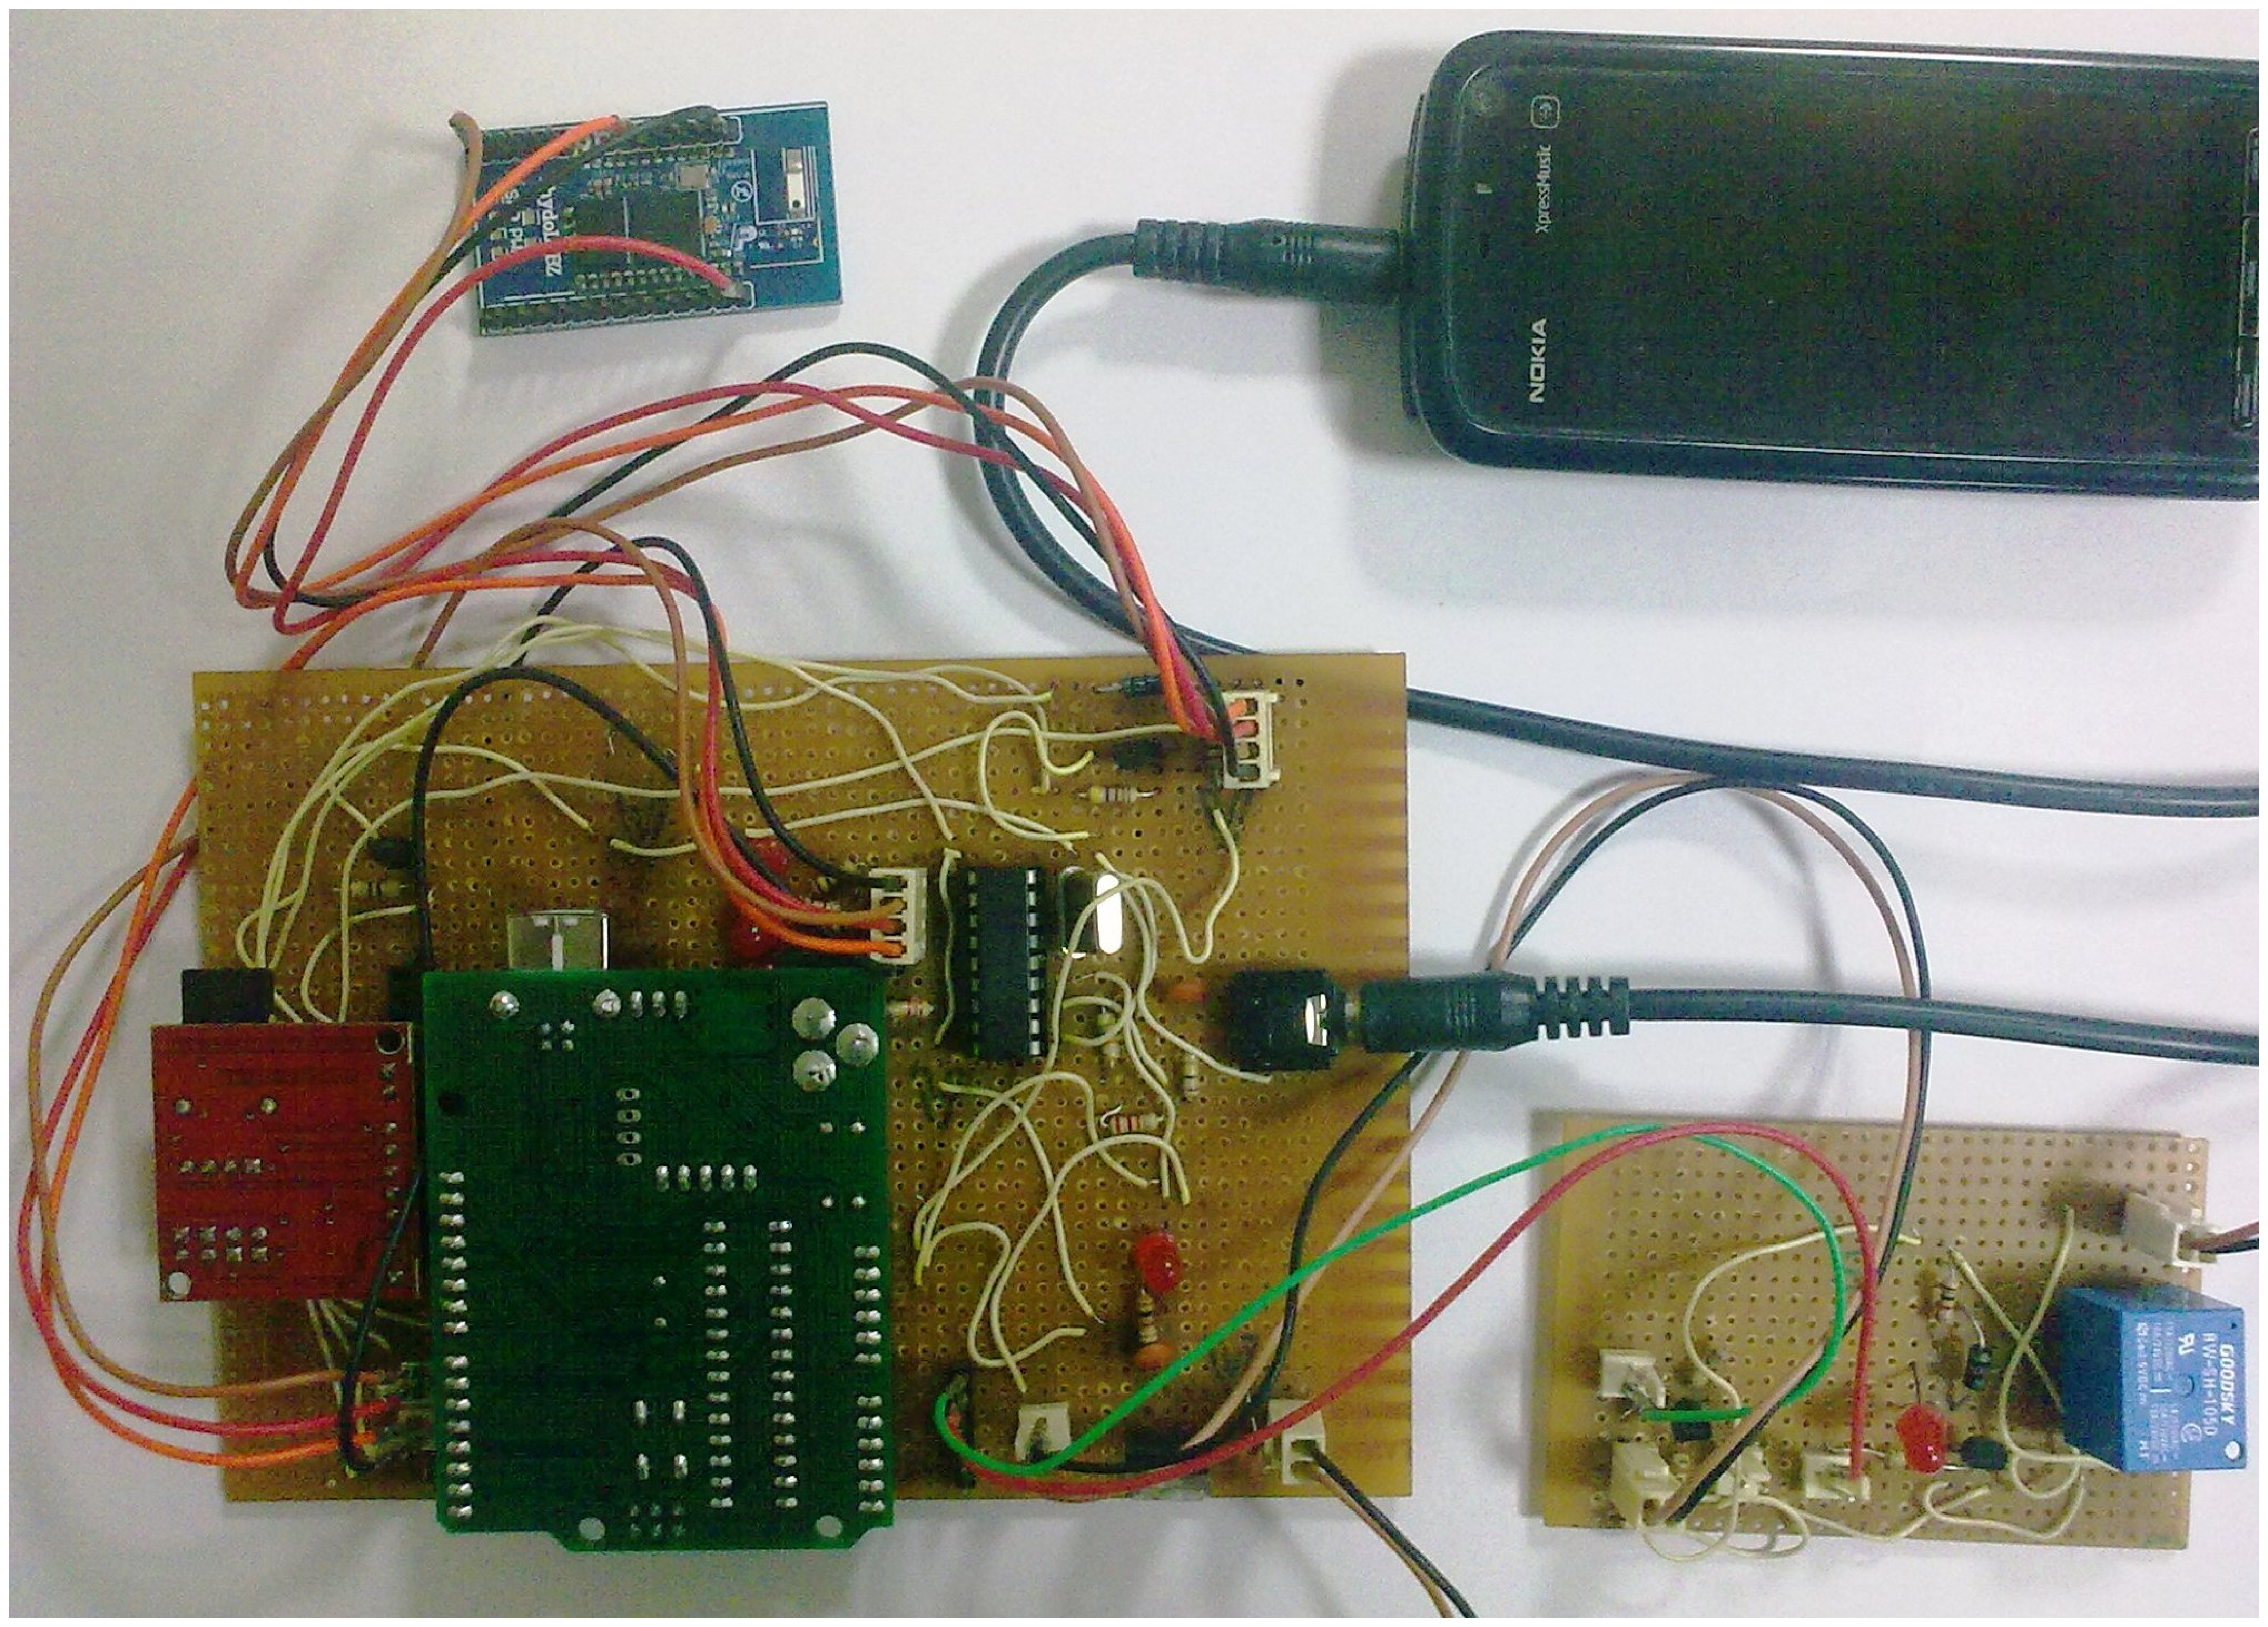
\epsfig{file=figs/melosboard.eps,scale=.12}
\caption{Prototype board of \melos with all components}
\label{fig:melosboard}
\end{figure}

\looseness -1
Phones at the lower end of the price spectrum do not possess similar capabilities as smartphones. The number and variety of embedded sensors is vastly reduced and they also lack a robust programming environment to develop applications that utilize in-built sensing capabilities. Moreover, interfacing any external sensors, as per application requirements, to mobile phones is also difficult\cite{psi} as most phones do not use standard communication interfaces such as UART, I2C, and SPI. Some phones use proprietary protocols by their respective vendors thus making it challenging to design a standard platform that can interface across broad category of low cost mobile phones. Such constraints necessitates a low-cost sensing extension for the mobile phone that can help bridge this gap and provide even low-cost phones with a sensing capabilities that can enable their use in broad range of applications. The extension should be programmable, have standard interface for sensors, and have a communication channel to connect to majority of phones especially low-cost phones. Moreover, it is essential that the system consumes low power to enable longer deployment periods for sensing. For example,~\cite{littlerock}presents a system which offloads the continuous sampling and processing operations to a low-power sensing attachment to reduce energy consumption.

\looseness -1
In this paper, we present a low-energy and low-cost generic sensing attachment \melos that attaches to a mobile phone through its audio port and is capable of attaching any external sensor, local storage, and controlled high bandwidth communication for data transfer. \figref{fig:melosboard} shows a photograph of the prototype of \melos platform. The ubiquity of the audio port in mobile phones makes it compatible with a large range of mobile phones. \melos can connect up to 6 external sensors as per application requirements. \melos also allows fine-grained switching control of on-board communication and storage devices thus reducing the total energy consumption. The total cost of \melos platform for single node from off-the-shelf components is approximately 65 USD. Simply with scale and using the necessary ICs in place of off-the-shelf breakout boards, the cost can significantly come down by a big factor. 

%Previous sensing platforms, like LEAP~\cite{LEAP}, have developed custom software and hardware to minimize power consumption. Also, mobile attachments like FoneAstra~\cite{foneastra} and HiJack~\cite{hijack} aim to enhance the sensing capabilities of mobile phones. \melos aims to combine both these aspects and provides an architecture that augments a mobile phone's sensing capabilities as well as consumes minimum power.

\looseness -1
\melos takes control information in the form of DTMF (Dual Tone Multiple Frequency) tones from locally connected mobile phone. The control information can be provided remotely both using SMS and audio call based network interfaces from a remote mobile phone to the local mobile phone. At the heart of \melos node is an AVR microcontroller. The microcontroller takes input in the form of DTMF tones to process the commands mapped to the corresponding tones. We demonstrate commands for switching on-board modules (Bluetooth communication and memory interface) for low power operation, switching external appliances using on-board relay, and switching the on-board ADC to start sensing the necessary parameters. We prototype a sample application to monitor energy consumed by an incandescent bulb and also demonstrate appliance control using a relay based circuit incorporated in \melos .  

\looseness -1
In summary, the key contribution of our work is a generic mobile phone extension platform that connects to any mobile phone over standard audio and Bluetooth interface. We minimize power consumption of the platform by providing fine-grained control of various system components. We further extending the capabilities of the platform to switch external appliances and allow for remote command input over both SMS and simple voice call over cellular network. 

\looseness -1
The rest of the paper is organized as follows. \secref{sec:rw} reviews the related systems and explores the pros and cons of existing systems. In \secref{sec:sysDes}, we present both the software and the hardware architecture of \melos platform, followed by discussing its various components and different modes of operation. \secref{sec:sysDes} also presents the evaluation of \melos. A case study of \melos for energy monitoring system is explained in \secref{sec:case} followed by conclusion and future work in \secref{sec:conc}.
%In section 5, we discuss the future work where we explains possible ways to extend it.

\section{Related Work}
\label{sec:rw}
\looseness -1
Low power consumption for long lifetime has been a key requirement in many of the sensing applications. Several approaches have been used in the past to reduce the overall system power consumption including switching the modules off as per application requirements. As an example, LEAP~\cite{LEAP} allows low energy operation while supporting for high computing operations through using two tier approach for both computing and communication. A low energy computing (and communication) device is used in ``always-on" state. A high-energy device is turned on when required to reduce the overall energy consumption per computation (or per byte transferred). We use a low power microcontroller in our \melos platform. For communication, we use the low-energy audio interface in ``always-on" state while turning high-bandwidth, high-energy Bluetooth interface as per requirements. We also control switching on-board memory module as per requirements to further reduce the overall system power consumption. 

\looseness -1
Several platforms have also been proposed in the past ~\cite{psi,nsmarts,smartconnect,foneastra,hijack} extending capabilities of mobile phones for sensing applications. However, most of them are designed for higher end mobile phones. \cite{psi} realizes a phone-centric body sensor network which requires a mobile phones'  SD/MMC card slot for external interface. However, there is no focus on reducing the overall power consumption of the platform. Similarly, \cite{nsmarts} - a mobile extension for air pollution monitoring also relies on higher end GPS enabled mobiles for operation and uses Bluetooth for external interface that consumes significant power during operation. 

\looseness -1
Similar phone extensions that extend the sensing capabilities of mobile phones include FoneAstra~\cite{foneastra} and HiJack~\cite{hijack}. One of the limitations of FoneAstra is that it uses Nokia's proprietary FBUS protocol for communication between the phone and platform. Moreover, the pop port that is used for communication is only available on only some of the low end Nokia phones and is not available on most other phones. This limits the use to only a small set of mobile phones. Since \melos interfaces with a mobile phone over standard audio port and Bluetooth interface and hence is generic enough to work not only with Nokia but with a wide variety of mobile phones as well. 

\looseness -1
HiJack uses iPhone's audio port for two-way communication between the phone and the sensing attachment. It consists of a microcontroller to generate coded signal that can be sampled by phone's microphone but need to be decoded by software running on the phone. Thus, only high end mobile phones that a have programming environment can be used to establish two-way communication between the phone and HiJack.

\begin{figure}
\centering
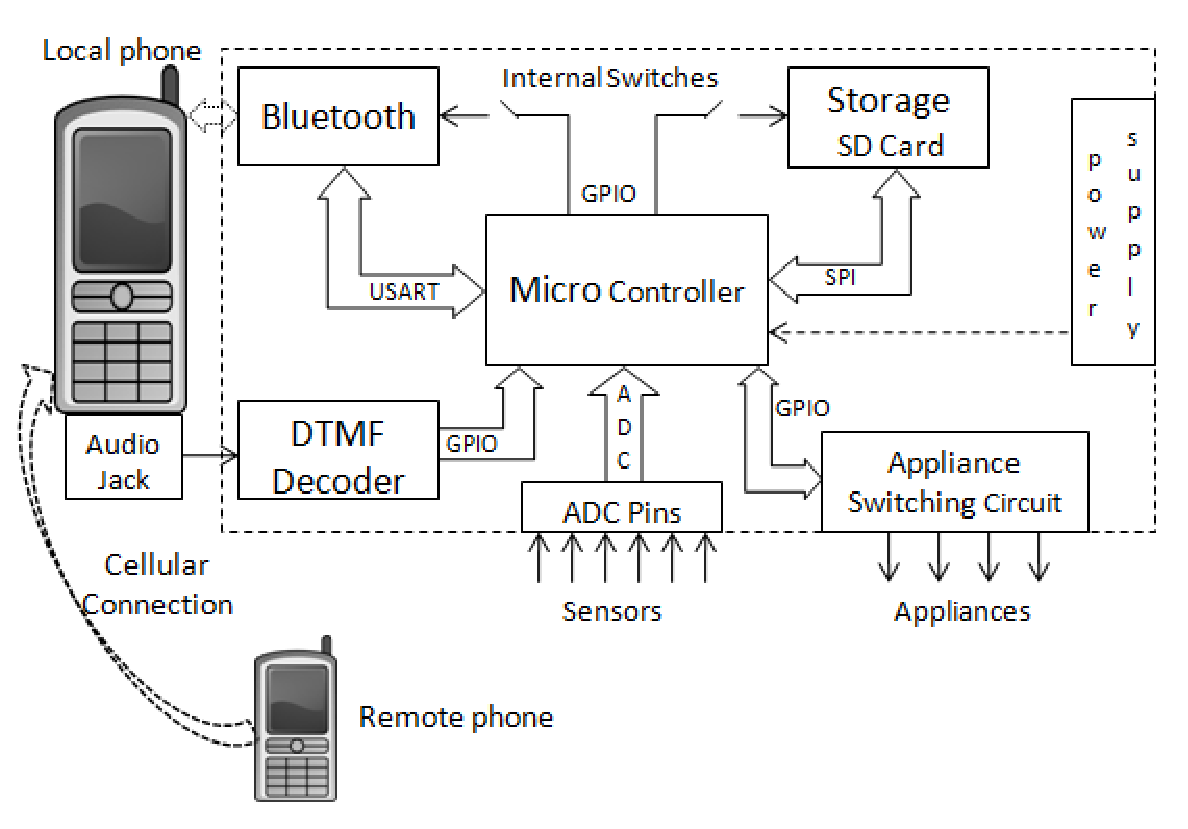
\epsfig{file=figs/blockdiagram.eps,scale=.43}
\caption{Architectural diagram of \melos node}
\label{fig:blockdiagram}
\end{figure}

%\begin{comment}
%HiJack uses iPhone's audio port for two-way communication between the phone and the sensing attachment. The audio port used for interface is unique to high-end Apple mobile devices (iPhone, iPod, and iPad) providing left, right, and microphone channels \redcolor{Are you sure? My headphone from iPod works on standard audio port as well.}. HoJack uses the right channel  for harvesting power for the device from the phone. The left and microphone channels are used for UART communication with the on-board microcontroller. Therefore, in functionality the audio port differs in usage from a standard 3.5 mm port that consists of standard TRS (Tip, Ring, Sleeve) bands and do not have a microphone channel. HiJack needs to be adapted for use with low-cost phones prevalent in developing regions.
%\end{comment}

\looseness -1
\melos provides a generic low-power system for sensing that can be attached to a mobile phone over standard audio interface. We provide fine-grained control of on-board modules and selection of different power modes to facilitate low-power sensing. The uniqueness of our proposed system lies in merging the ubiquity of mobile phones with low-power consumption thus enabling a large number of potential applications (energy monitoring, healthcare, etc) over a long deployment period.

\section{System Design and Evaluation}
\label{sec:sysDes}
\looseness -1
Hardware design typically entails a trade-off between overall system cost (and other parameters such as power consumption) and time to develop a prototype platform. For our \melos prototype platform, we are currently using off-the-shelf hardware attachments for several modules involved in the design (such as Bluetooth communication and external memory interface) that helped us reduce the time to develop a working platform. Further, using external hardware attachments also results in increased power consumption for the overall system due to additional ICs incorporated on each of these attachments. Even with such an approach of using multiple off-the-shelf hardware attachments, the overall system cost as well as system power consumption is small. We believe that a customized hardware design with required components laid out on a single board will reduce the overall cost as well as the power consumption by a significant factor from the current values. Next, we explain the hardware architecture of \melos in detail followed by different modes of operation and evaluation of the system for overall power consumption.

%\begin{comment}
\begin{figure}
\centering
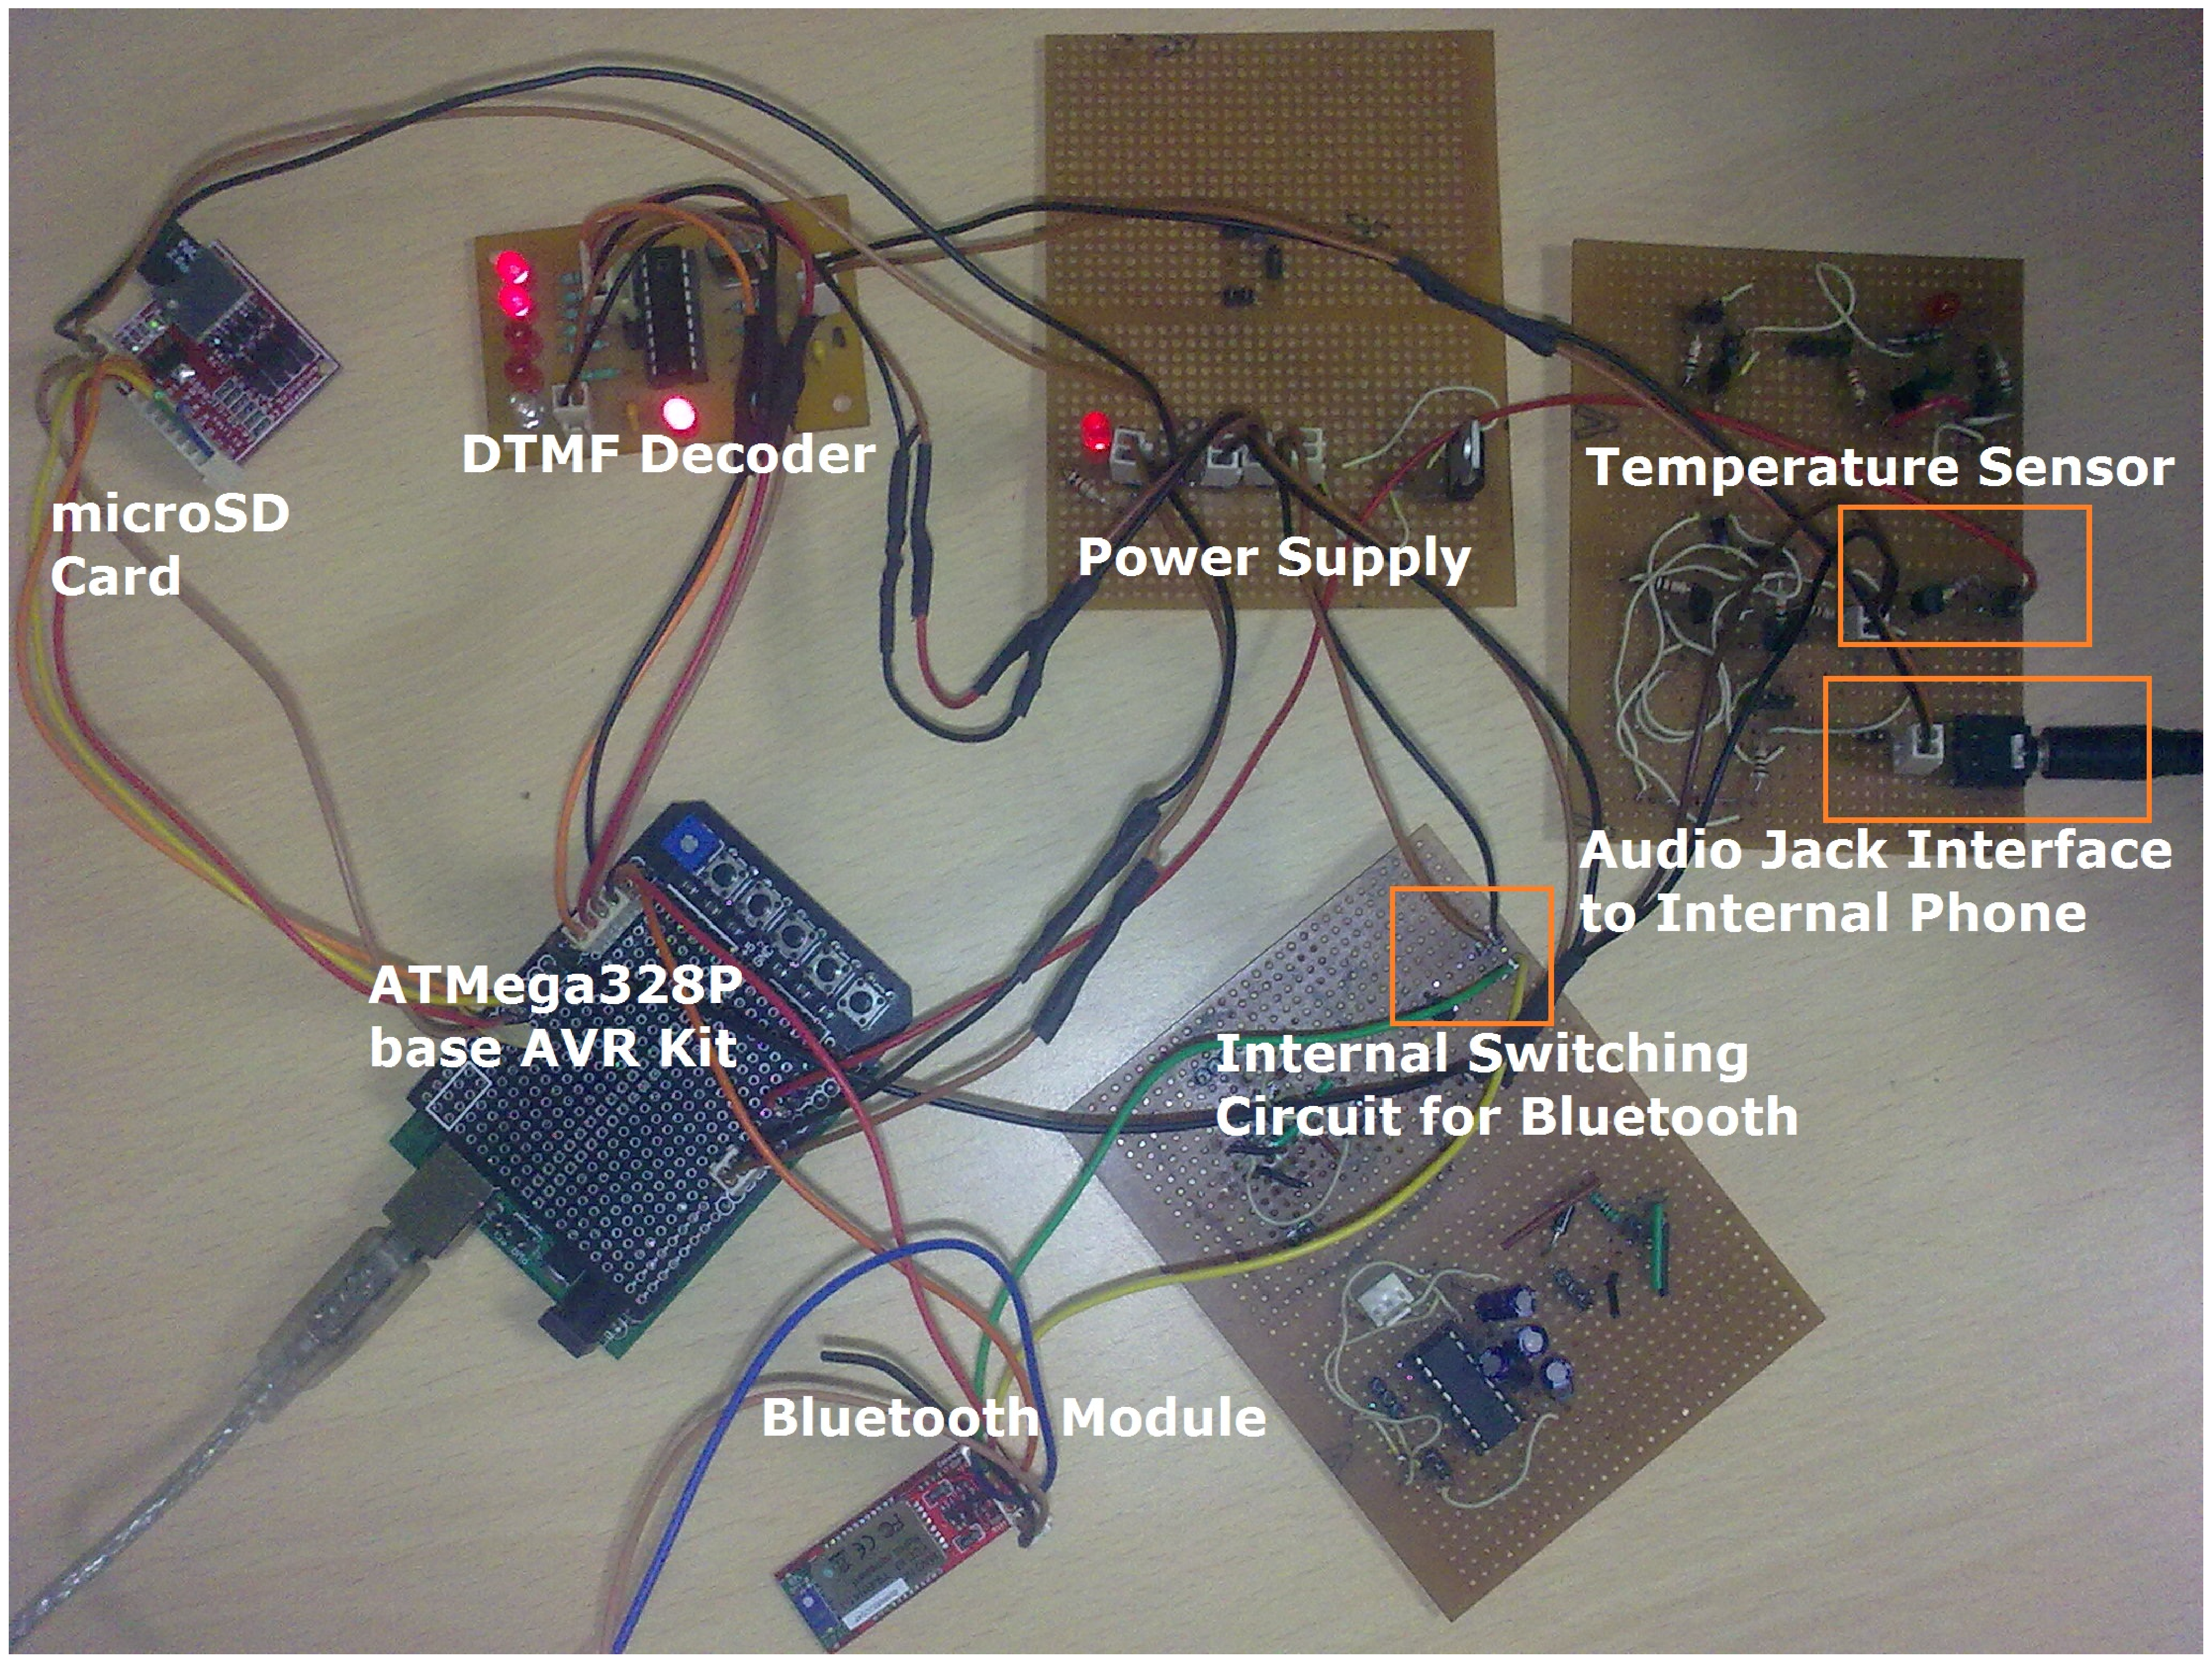
\epsfig{file=figs/meloscircuit.eps,scale=.12}
\caption{Different modules of \melos node wired together}
\label{fig:meloscircuit}
\end{figure}
%\end{comment}

\subsection{Hardware Architecture}
\looseness -1
\figref{fig:blockdiagram} displays the architectural diagram of \melos node. The platform interfaces with a local mobile phone over the audio interface using a standard 3.5 mm audio jack. Communication with a local mobile phone over the audio port works as a one way communication from the phone to the platform wherein different commands can be send from the phone to the node using DTMF tones. The advantage of using the audio port for interface are three folds - 1. It is a standard interface across phones from all manufacturers and across all price range; 2. Even a non-programmable phone (with auto-answer capability) can be used as an interfacing device to receive the commands from a remote mobile phone over the cellular network; 3. Audio interface consume insignificant power when in standby mode thus ensuring low power ``always on" interface between the phone and the \melos node. 

\looseness -1
A connection can be setup between the remote mobile phone and the local mobile phone using SMS or audio call to pass on multiple commands from the remote location to the \melos node over ubiquitous cellular network. With inexpensive call and SMS rates available in developing regions, such a connection ensures low cost command passing interface remotely to a \melos node. In case of a voice call DTMF tones as received by the local mobile phone are passed on to the \melos node. For SMS, we create an application that can parse the SMS to produce the DTMF tones accordingly for the \melos node. A DTMF decoder is used on the \melos node to decode the commands. We use Zarlink Semiconductor's MT8870D\footnote{\url{www.zarlink.com/zarlink/hs/82_MT8870D.htm}} IC for decoding DTMF tones because of its low-power consumption and TTL output corresponding to binary value of each key press. The IC also provides an option of a power down pin that can be used to further reduce the power consumption of the node by inhibiting the operation of the DTMF decoder chip, if desired.

\looseness -1
At the heart of \melos node is Atmel's ATmega328P\footnote{\url{www.atmel.com/dyn/products/product_card.asp?part_id=4198}} microcontroller. There are multiple advantages of using ATmega328P microcontroller: 1. It provides several low power modes of operation with low standby power of less than 1 $\mu$A and active power consumption of 0.2 mA; 2. It is readily and cheaply available; 3. It can be easily programmed using C environment; 4. Six on-chip Analog to Digital Converters (ADCs) that can be used for sensing multiple parameters; 5. In-built USART for serial communication with on board peripherals (Bluetooth module and external memory interface); and 6. Enough on-chip memory (1KB EEPROM, 32 KB Flash) for storing sensed values. The microcontroller takes input from DTMF decoder to process the commands mapped to the corresponding DTMF tones. These commands include switching on-board modules (Bluetooth communication, memory interface) for low power operation, switching external appliances using on-board relay, and switching the on-board ADC to start sensing the necessary parameters. 

\looseness -1
The microcontroller supports six 10-bit on-chip ADC channels. DTMF tones are used to start sensing on these ADC channels. The sensed data is stored in the on-chip memory and periodically transferred to the external memory. The frequency of transfer is decided based on frequency and volume of sensed data to reduce the overall system power consumption. Since external memory consumes significant amount of power, it will be switched on only when data transfer is required and will be switched off remaining time. For example, if a temperature sensor is attached to \melos and the data logging frequency is 1Hz, by taking the mean value of higher frequency sensing, then approximately once in every 85 minutes external memory will be switched on and readings will be transfered from internal data memory to external memory.  We use a breakout board\footnote{{\small\url{www.embeddedmarket.com/products/Micro-SD-card-Interface-Breakout-Module-for-3-3V-and-5V-Logic-Level}}} to interface a microSD card to our device. The card is connected to the microcontroller over SPI (Serial Peripheral Interface). With low cost high capacity microSD cards easily available, the total memory capacity of the system can be enhanced as per the application requirements. Data stored in the microSD card can be retrieved by physically detaching the SD card as well as over Bluetooth interface. 

\looseness -1
To collect the sensed data remotely, a Bluetooth module is used to communicate sensor data from the microcontroller to the local phone. Data from the local mobile phone can then be sent to a remote location over cellular network (SMS/GPRS). Bluetooth connection provides the return connectivity from the \melos node back to the local mobile phone. We use off-the-shelf BlueLINK Bluetooth\footnote{\url{www.rhydolabz.com/index.php?main_page=product_info&products_id=454}} module that supports a large variety of baud rates ranging from 9600 to 115200 and has a multiple low power modes with variable sniffing time that can be easily configured using AT commands. Communication between microcontroller and Bluetooth module takes place over a serial link (UART). Since Bluetooth communication consumes significant power (approximately 70mA) during communication , a remote user can send a command to local mobile phone for switching the Bluetooth module as per requirement to reduce the overall system power consumption. The command is then passed on over the low power "always on" audio interface using DTMF tones and processed and acted upon by the microcontroller. When turned on, the sensed data from microSD card is transferred to the local mobile phone over high bandwidth Bluetooth connection at 9.6Kbits/s. Burst transmission over Bluetooth results in achieving small energy consumption of approximately 208$\mu$W per byte transferred.

\looseness -1
\melos also supports on board relay modules to control switching of external electrical appliances. The relay switch is connected to GPIO pin of the microcontroller. A command to switch the external appliances can be issued by a remote user that is passed on over cellular network to the local mobile phone and then on to the microcontroller using the DTMF tones. For the energy monitoring application, on-board relays provide capability to switch the electrical appliances as per requirements in addition to sensing the required parameters (such as current consumption, and temperature among others).  

\looseness -1
\melos is powered by an external battery or an adapter (between 6-18V DC). We use a low cost voltage regulator 7805 to generate 5V from the external supply. All peripherals and the microcontroller operate on 5V supply voltage. The break-out boards used for SD card and Bluetooth module are 5V compliant thus obviating the need of level converters. \figref{fig:meloscircuit} displays a picture depicting different modules of \melos node wired together. The picture is only for illustration purpose; for the prototype node, we have connected these modules on a single board as illustrated in \figref{fig:melosboard}. Next,  we discuss different modes of operation possible with \melos board that can be used to optimize the overall energy consumption for a given sensing application.





%\begin{comment}
%\begin{table}
%\centering
%\caption{Different modes of operation}
%\begin{tabular}
%{|c|c|l|c|} 
%\hline
%Module&Mode& Current & Power\\ \hline
%Bluetooth & Not Connected but On & 30mA & 150mW\\ \hline
%Bluetooth & Transferring data & 50mA & 250mW\\ \hline
%SD Card & Write/Read data & 60mA & 300mW\\ \hline
%DTMF Decoder & On and Active & 3mA & 15mW\\ \hline
%DTMF Decoder & Standby & 10uA & 50uW\\ \hline
%\end{tabular}
%\end{table}
%\end{comment}
%
\begin{table*}
\centering
\begin{tabular}
%{|c|c|l| p{1.5cm}|c|} 
{|c|c|c| c|c|c|c|c|} 
\hline
Mode &Controller Kit& Bluetooth & SD Card & DTMF Decoder & Miscellaneous & Total rated power & Measured power\\
 (Power) & (100mW) & (230mW) & (300mW) & (15mW) & power (mW) & (mW) & (mW) \\ \hline
Stand by & On & Off & Off & On & 100 & 115 & 235 \\ \hline
Data logging & On & Off & On & On & 165 & 415 & 500\\ \hline
Data Transfer& On & On & On & On & 165 & 645 & 400-700\\ \hline
\end{tabular}
\caption{Total rated power and Measured power for different modes of \melos. Power consumption of passive components and sensor is listed as Miscellaneous power}
\label{table:modes}
\end{table*}

\begin{figure*}
\centering
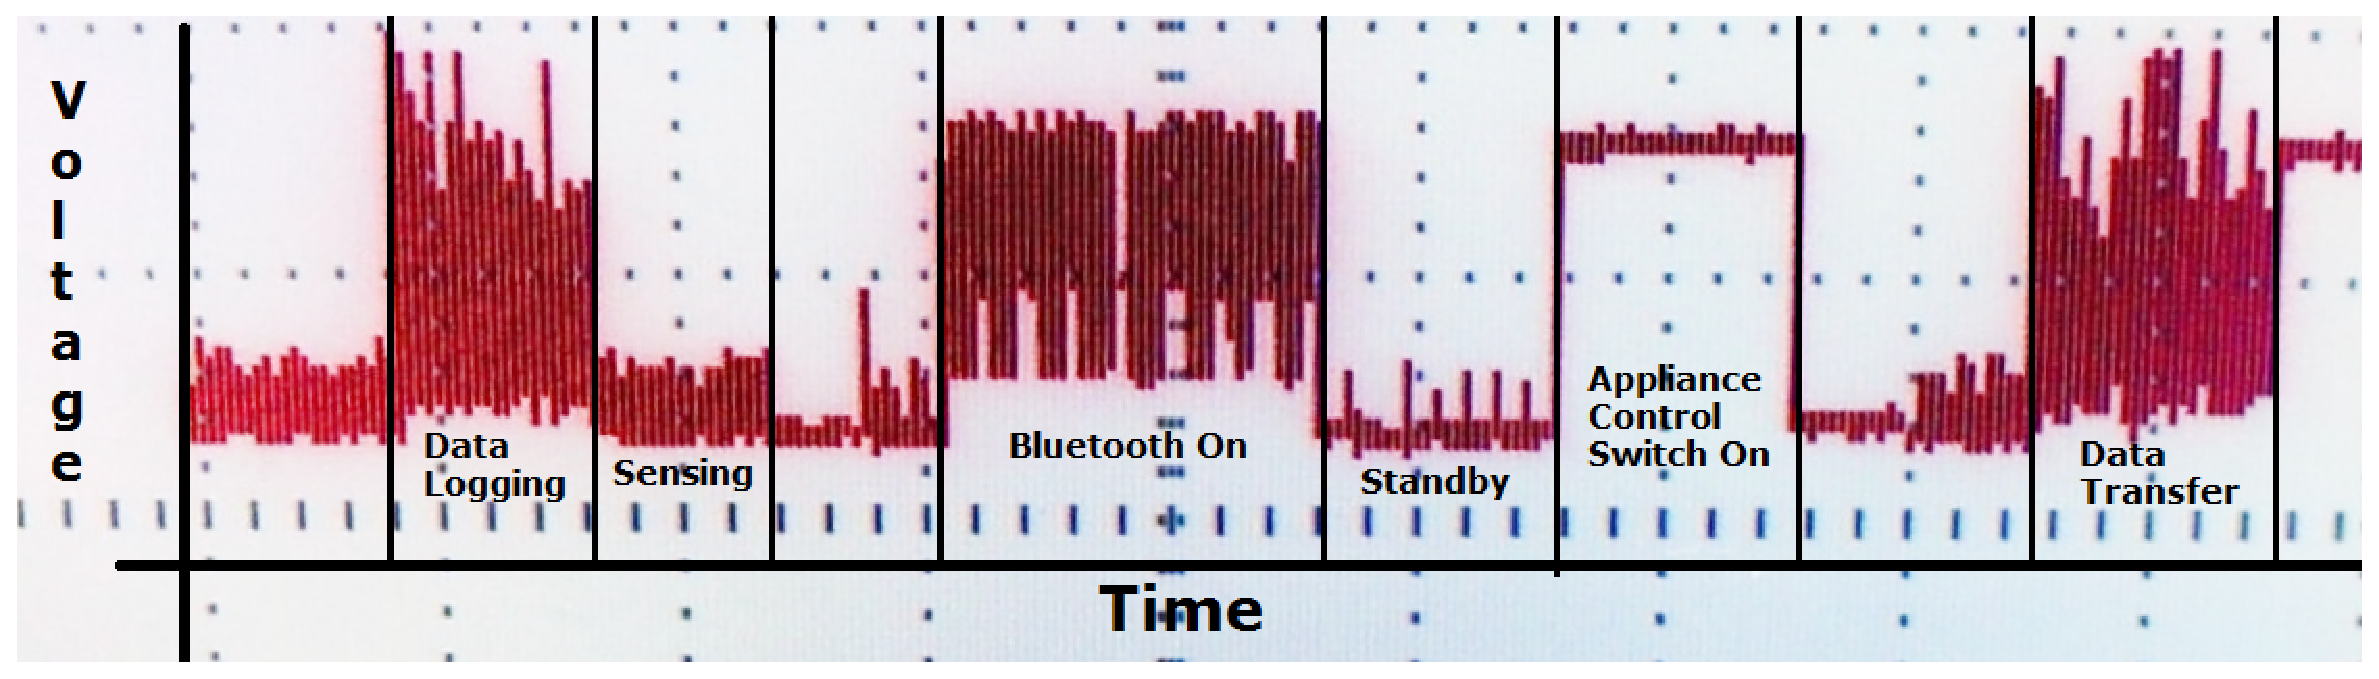
\epsfig{file=figs/oscilloscope.eps,scale=.4}
\caption{Voltage readings from Oscilloscope for different modes \melos \redcolor{needs to add the precise voltage range}}
\label{fig:oscilloscope}
\end{figure*}

\subsection{Modes of Operation}
\looseness -1
We divide operations of \melos into three primitive modes - Standby, Data Logging, and Data Transfer. The Standby mode is disjoint with other two modes. The last two modes are not disjoint. In other words, \melos could be in a mode, which is a combination of Data Logging and Data Transfer. \figref{fig:statetransition} displays the state transition diagram and shows the state and operations of data logging and data transfer mode of \melos with respect to commands from the user. Active components and corresponding total power consumption of each mode is specified  in \tabref{table:modes}. 

\begin{figure}
\centering
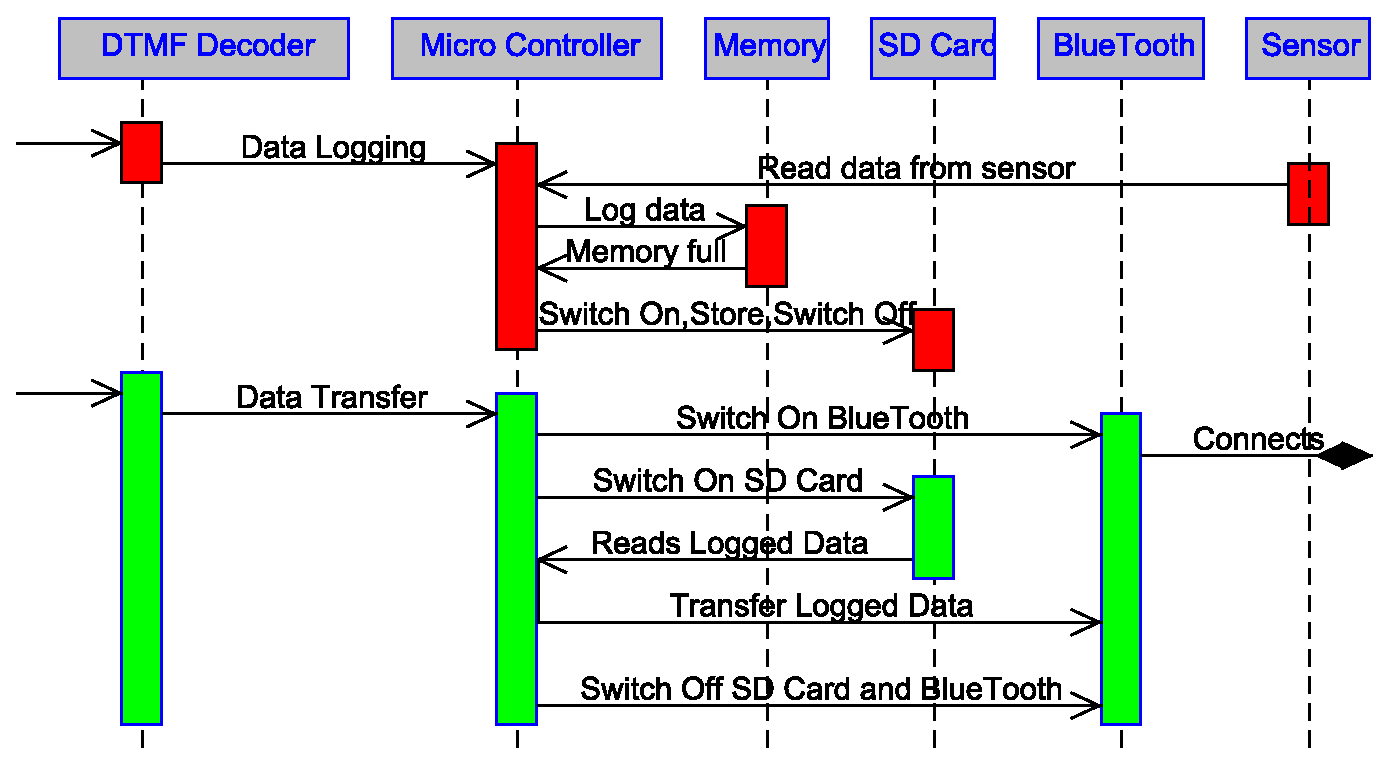
\epsfig{file=figs/statetransition.eps,scale=.36}
\caption{Transition diagram for Data logging and Data transfer mode of \melos}
\label{fig:statetransition}
\end{figure}

%\ohm
\looseness -1
To evaluate the power consumption for each mode we connected a 10Ohms resistor in series to the power supply of \melos. Then we measured the voltage across this resistor using oscilloscope from which we calculated the current consumption. \figref{fig:oscilloscope} shows the plot of voltage change for each mode of \melos . The measured power in  \tabref{table:modes} includes the power consumption of few passive components we used on the board. Also, the microcontroller kit consumes 100mW because it has inbuilt FTDI IC and few more passive components. All these passive components power can be reduced if we design \melos on single board. An overview of different mode, various operations, state of each module, total rated power and measured power for each module is explained in detail below.  

\subsubsection{Standby Mode}
\looseness -1
This is the initial and the default mode of \melos . After powering up or reseting the node, the microcontroller initializes all sub modules connected to \melos and goes to the Standby mode. In Standby mode, no operation is performed and the microcontroller keeps on waiting to receive control information. All modules are powered down except the DTMF decoder, from which, the control information is received. Depending upon the control information received from DTMF decoder, \melos goes to either Data Logging or Data Transfer mode. The total rated power consumption in standby mode is power consumption of microcontroller kit and DTMF decoder on the board, which is about 115mW. The measured power in standby mode is 235mW including the the power consumption of passive components.

\subsubsection{Data Logging Mode}
\looseness -1
When the user sends control information to activate a particular sensor, \melos goes into Data Logging mode. Unique control information is used to activate or deactivate each of the ADC channels inside the microcontroller. Once a particular sensor is activated, data logging begins at a predefined frequency. By default, all sensor readings are stored temporarily in on-chip memory. Once all available on-chip memory is full, SD card module will be switched on and all data from local memory will be transferred into SD card. As a result, SD card module need not be active all the time. It reduces the overall average current consumption of SD card module.

\looseness -1
In the Data Logging mode, the total rated power consumption is the consumed power for microcontroller kit, DTMF decoder and SD card. Thus, the total power consumption is 115mW, when data is logged into internal memory and 415mW when writing data to SD card whereas the measured power is 500mW. The miscellaneous power includes the power consumption of passive components and active sensor. Depending upon the next control information received from user, \melos either goes to Standby or Data Transfer mode.

\subsubsection{Data Transfer Mode}
\looseness -1
\melos goes into Data Transfer mode when user wants to transfer the logged data from the SD card to another device, which could be a mobile phone or laptop with Bluetooth support. Once it receives the unique control information for data transfer, Bluetooth module is switched on. The Bluetooth module will be in listening mode to accept connection from other Bluetooth enabled devices to which data is to be transferred. After establishing the connection, microcontroller switches on the SD card module, if it is not already switched on. Then, the microcontroller starts sending the logged data via Bluetooth as a data stream. Maximum power is consumed in this mode as all the modules of \melos are switched on and functioning. The total rated power consumption of this mode is about 645mW and measured power consumption is between 400 to 700mW which is depends upon the duration of  Bluetooth connection establishment.

\section{Case Study : Energy Monitoring}
\label{sec:case}
\looseness -1
Energy consumption in residential and commercial buildings, account for a significant percentage of total national consumption across the world.  Even a small percentage reduction at building level can have significant additive impact in reducing the overall consumption. A system that allows fine-grained monitoring of energy consumption of appliances can give a great insight into the consumption during different time-intervals in the day. This information can then make the user aware of an optimum usage pattern that
can minimize the overall power consumption.

\looseness -1
\melos act as a platform that can both remotely control appliances as well as monitor the energy consumed by each appliance using ubiquitous cellular network. We interface a current sensor ACS714\footnote{\url{http://www.rhydolabz.com/index.php?main_page=product_info&products_id=506}} that can  measure bidirectional current in the range -5A to +5A . The appliance to control and monitor is connected in series with the current sensor and the switching relay (driven by one of the GPIO pin of the microcontroller). Using DTMF tones passed on as a command from a remote phone (over SMS/audio call), the control information is passed to the microcontroller to turn on the appliance and start sensing the current.

\begin{figure*}
\centering
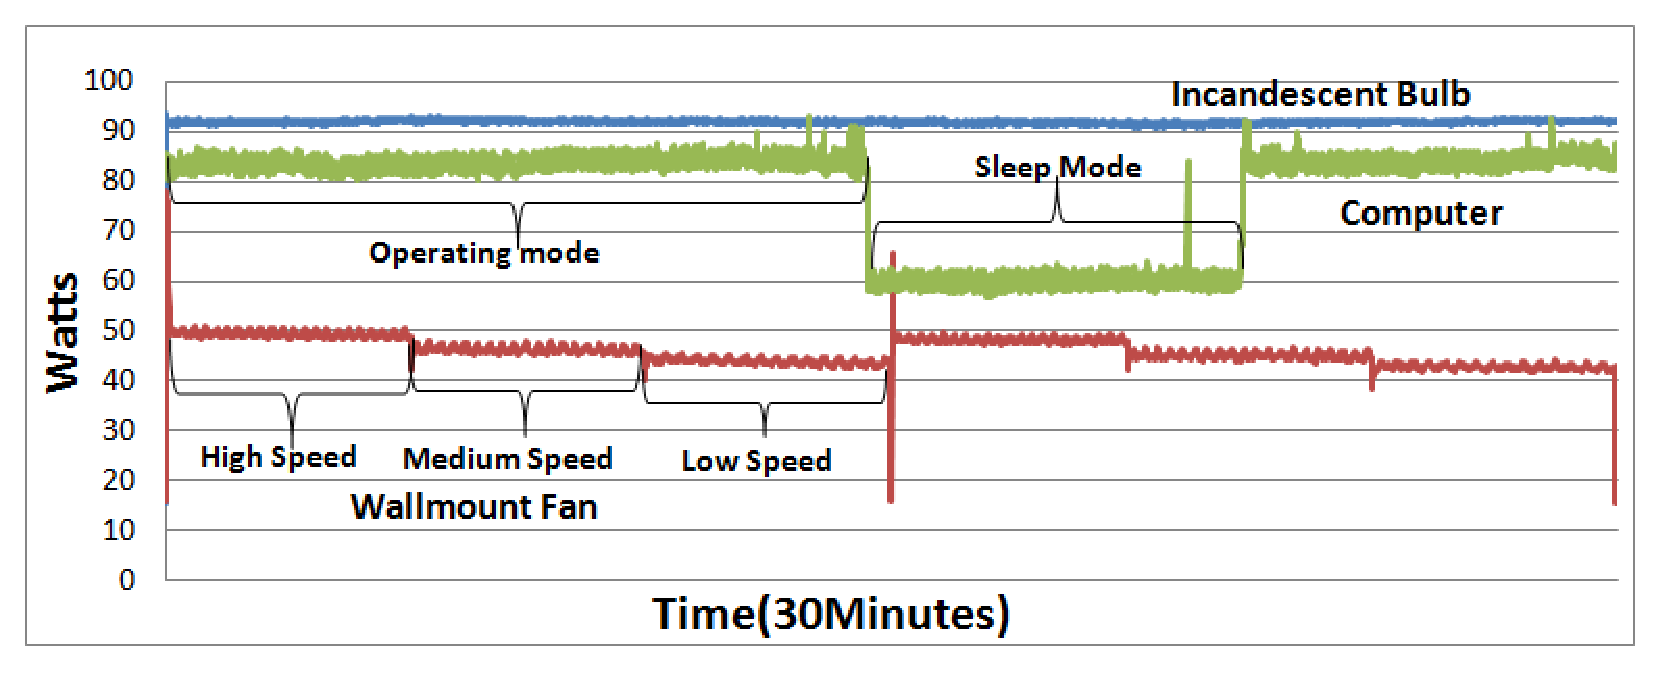
\epsfig{file=figs/energychart.eps,scale=.55}
\caption{Energy consumption of Incandescent bulb, Wall-mount Fan and Computer which also shows modes of each appliance }
\label{fig:energychart}
\end{figure*}

%\begin{comment}
%For the sake of simplicity, we assumed the bulb acts as a purely resistive load. We used the ADC interrupt to read the samples of current consumed by the light bulb. Then with 220V as the Root Mean Square (RMS) voltage consumption of the bulb , the current consumed by the bulb is 181 mA. Our setup returns the current consumed by the bulb as \redcolor{XX}mA which corresponds to power consumption of \redcolor{YY}Watts indicating an error of \redcolor{ZZ}\%
%\end{comment}

\looseness -1
\figref{fig:energychart} shows the plot of energy consumption of three appliances: An incandescent bulb,  wall-mount fan and computer as monitored by the \melos node. Current sensing observations were collected in the local memory and passed on to the computer over Bluetooth. A negative spike in the plot for the computer happened when it went to sleep mode. For wall-mount fan, we manually adjusted the speed to measure the power consumption in each state. 
%With valid assumptions, we compared each appliance's measured power with their rated power to know the error rate which was around 6\%. 
Together with current sensing, we can also have a diode based full wave AC to DC rectifier circuit, followed by a step down converter to measure the voltage consumed by the load using the ADC ports available on \melos . Furthermore, we can also use zero-crossing detectors to measure the power factor thus giving a more accurate idea of power consumption of each load. Using on-board relays, switching of external appliances can also be performed easily using \melos node. This switching can be either manually controlled (through commands passed using remote mobile phone) or can also be automated based on sensor observation as performed by the \melos node. The setup can be easily extended to monitor home and office premises by attaching sensors like motion, light, vibration, and gas, among others.

%\begin{comment}
%We present a case study where we use \melos
%to measure temperature and control switching on and off of an incandescent light bulb.
%We used both audio and SMS channel to control the operation of \melos .
%
%We used LM-35 temperature sensor for its low cost, large range (0-100 C), and easy of interfacing with our microcontroller. 
%We connected the audio output of ??xyz 5130?? phone to \melos' audio 
%input jack and the phone was put in auto-answer mode. We attached the LM35 temperature sensor to 
%one of the ADC channel. Also, we attached a 40W incandescent light bulb via Omron SPST Relay 
%circuit, which is driven by one of the GPIO pin of the microcontroller. Each unique DTMF tone was 
%mapped to control a particular component. We configured, DTMF tone 1 and 2 to switch on and off 
%temperature sensor, DTMF tone 3 and 4 to switch on and off Bluetooth module and DTMF done 5 and 6 to switch on and off the incandescent light bulb. \melos 
%is powered up using ??xyz??.
%We placed a call from another mobile to the mobile attached to 
%\melos . Once the call is connected, we pressed the respectively mapped keys to send DTMF tones to control 
%different functionalities of \melos . 
%
%We also experimented another setup to control the \melos using SMS messages. For this setup, a higher 
%end ??xyz 5800?? was connected to \melos . The Bluetooth on the phone is switch on initially. We deployed a Python program 
%on the phone that interfaces with SMS and Bluetooth.
%Depending upon the content of the SMS, the Python program plays an mp3 file of the DTMF code.
%
%\begin{comment}
%At the beginning of execution, this module binds a callback function to an event which is 
%generated by any incoming message. Whenever a new message arrives, the callback gets called; it 
%reads that message and validates the control information. (Sender authorization can be added such 
%that it can proceed further only for a particular user's SMS). Whenever a new SMS arrives, it 
%validates and extracts the control information character which is expected in first character of 
%the SMS. Then it searches the corresponding control information code's DTMF tone mp3 file which 
%was already stored in mobile and plays it. Also, if the control information is to switch on 
%Bluetooth module, it waits for 3 seconds to let the microcontroller to switch on Bluetooth module, 
%searches and connects to the pre-configured Bluetooth module which is connected to the system. 
%Once connected, it receives and stores the readings data from the Bluetooth.
%We verifed the temperature and the power measure by \melos are indeed correct.
%\end{comment}
%
%\begin{comment}
%\subsection{Energy Monitoring}
%\melos is also capable of measuring the energy consumed by appliances. We use a current sensor connected to the ADC of the microcontroller and our program calculates the RMS value of the current consumed by the appliance.
%
%\subsection{Appliance Control}
%\melos possesses the capability to switch individual devices (/home appliances) based on the control information sent by the user. We use a Relay connected to a GPIO pin of the microcontroller to switch devices using the output of the microcontroller.
%
%\subsection{Environmental Monitoring}
%\melos can also be used to monitor the environment by attaching various sensors  such as temperature ,humidity  and gas concentration sensors to the ADC port of the microcontroller. It is capable of supporting upto six sensors attached together to the ADC and can thus monitor the environment comprehensively. For testing we attach the LM-35 temperature sensor and log the room temperature values to the on board SD card. We can also have a real-time plot of the temperature sensor data as seen on the figure below.
%
%\end{comment}

\section{Conclusions and Future Work}
\label{sec:conc}
\looseness -1
Low cost and low energy sensing attachments for low end mobile phones can significantly enhance their capabilities for use in critical sensing applications such as energy monitoring and environmental sensing. In this paper, we proposed a mobile extension called \melos, that interfaces with a mobile phone over generic audio and Bluetooth interface. The generic audio port is used as low-energy, ``always-on" unidirectional interface for passing the control information from the locally attached mobile phone to the \melos node. This control information can be used for multiple purposes - 1. Control switching the on-board memory and communication interface as per application requirements to further reduce the power consumption of the \melos node; 2. Control switching of external appliances using on-board relays; 3. Initiate sensing of necessary parameters.
We discuss the hardware architecture and various modes of operation illustrating reduced energy consumption of the \melos node. We also present a case study for energy monitoring and appliance control system using \melos node. 

In the future we plan to perform extensive case studies for energy monitoring in buildings using \melos node. We plan to integrate other sensors, such as temperature, humidity, air-flow that can give accurate state information about the indoor environment using which automated switching of electrical appliances can be performed.

\section{Acknowledgment}
\looseness -1
We would like to thank Nokia Research Lab, Finland for funding part of the research for this project. We also acknowledge that the initial idea of using the audio port for mobile phone extension came from a product called Nano Ganesh used for remotely switching water pumps in agriculture domain.

\bibliographystyle{abbrv}
\bibliography{references}


\end{document}
